\chapter{Specialization}

%\section{Inheritance revisited}

When we first looked at inheritance in Chapter~\ref{eights}, our purpose was to avoid duplicating code.
We noticed that ``decks of cards'' and ``hands of cards'' had common functionality, and we designed a \java{CardCollection} class to provide it.
This design technique is known as {\bf generalization}.
By generalizing the code, we were able to reuse it in the \java{Deck} and \java{Hand} classes.

In Chapter~\ref{conway}, we looked at inheritance from a different point of view.
When designing \java{GridCanvas} to represent a grid of cells, we extended \java{Canvas} and overrode its \java{paint} and \java{update} methods.
This design technique is known as {\bf specialization}.
By specializing the code already provided by \java{Canvas}, we were able to draw grids on the screen with very little effort.

Notice that we didn't write the code for \java{Canvas}; it's part of the Java Library.
But we were able to extend it for our own purposes.
In fact, the \java{Canvas} class was specifically designed to be extended.

Throughout this chapter, we'll explore the ideas of inheritance and code reuse more fully.
We'll continue to develop graphical simulations as a running example, but this time, we'll draw varying shapes and colors.


\section{Polygon Objects}

The word polygon means ``many angles''; the most basic examples of polygons are triangles (3 angles), rectangles (4 angles), pentagons (5 angles), and so forth.
Polygons are an important part of computer graphics, because they are used to compose more complex images.

Java provides a \java{Polygon} class (in \java{java.awt}) that is relatively straightforward to use.
The following code creates the triangle shown in Figure~\ref{fig:triangle}:

\begin{code}
Polygon p = new Polygon();
p.addPoint(57, 110);
p.addPoint(100, 35);
p.addPoint(143, 110);
\end{code}

\begin{figure}[!ht]
\begin{center}
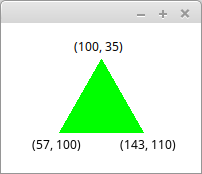
\includegraphics{figs/triangle.png}
\caption{A polygon with three points.}
\label{fig:triangle}
\end{center}
\end{figure}

Internally, \java{Polygon} objects have three attributes:

\begin{itemize}
\item \java{public int npoints;} {\tt ~~~} \java{// total number of points}
\item \java{public int[] xpoints;} {\tt ~} \java{// array of X coordinates}
\item \java{public int[] ypoints;} {\tt ~} \java{// array of Y coordinates}
\end{itemize}

%The \java{npoints} attribute makes it possible to add points to the polygon one at a time.
When a \java{Polygon} is created, \java{npoints} is 0 and the two arrays are initialized with length 4.
As points are added, \java{npoints} is incremented.
If \java{npoints} exceeds the length of the arrays, larger arrays are created, and the values are copied from the previous arrays.

The \java{Polygon} class provides many useful methods like \java{contains}, \java{intersects}, and \java{translate}.
However, it doesn't provide any methods for displaying the polygon like \java{draw} or \java{toString}.


\section{Adding Color}

Specialization is useful for adding new features to an existing class, especially when you can't (or don't want to) change its design.
For example, we can extend the \java{Polygon} class by adding a \java{Color} attribute and implementing a \java{draw} method:

\begin{code}
public class ColorPolygon extends Polygon {
    public Color color;

    public ColorPolygon() {
        super();
        color = Color.GRAY;
    }
    
    public void draw(Graphics g) {
        g.setColor(color);
        g.fillPolygon(this);
    }
}
\end{code}

As a reminder, constructors are not inherited when you extend a class.
If you don't define a constructor, the compiler will generate one for you that does nothing.
The constructor for \java{ColorPolygon} uses the \java{super} keyword to invoke the constructor for \java{Polygon}.
It then initializes the color to \java{GRAY}.

\java{ColorPolygon} has the same attributes and methods that \java{Polygon} has, in addition to \java{color} and \java{draw}.
You can use \java{addPoint} as before, or you can directly access \java{npoints}, \java{xpoints}, and \java{ypoints} (since they are \java{public}).
You can also use methods like \java{contains}, \java{intersects}, and \java{translate}.

The following code creates the same triangle as shown in Figure~\ref{fig:triangle} and sets its color to \java{GREEN}:

\begin{code}
ColorPolygon p = new ColorPolygon();
p.addPoint(57, 110);
p.addPoint(100, 35);
p.addPoint(143, 110);
p.color = Color.GREEN;
\end{code}


\section{Regular Polygons}

The original \java{Polygon} class has two constructors: one that creates an empty polygon, and one that copies existing values into \java{xpoints}, \java{ypoints}, and \java{npoints}.
%Creating arbitrary polygons with many sides is tedious work.
It would be nice if we could construct $n$-sided polygons without having to specify all the coordinates manually.

For simplicity, we'll focus on regular polygons, where all sides have the same length and all angles are equal in measure.
Regular polygons are a special case of polygons, so it makes sense to use specialization.

We could extend the \java{Polygon} class, like we did in the previous section.
But then we would lose the \java{Color} functionality we just added.
So we will make \java{RegularPolygon} extend \java{ColorPolygon}.

To construct a regular polygon, we will specify the number of sides, the radius (distance from the center to a vertex), and the color.
For example:

\begin{code}
RegularPolygon rp = new RegularPolygon(6, 50, Color.BLUE);
\end{code}

\begin{figure}[!ht]
\begin{center}
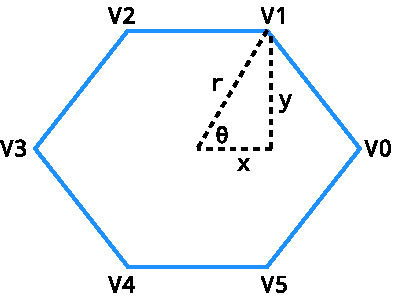
\includegraphics{figs/hexagon.pdf}
\caption{Determining the $x$ and $y$ coordinates of vertex V1, given the radius~$r$ and angle~$\theta$. The center of the polygon is at the origin $(0, 0)$.}
\label{fig:hexagon}
\end{center}
\end{figure}

The constructor uses a bit of trigonometry to find the coordinates of each vertex.
The number of sides ($n=6$) and the radius ($r=50$) are given as parameters.
Figure~\ref{fig:hexagon} illustrates the process:

\begin{itemize}
\item Imagine a clock hand starting at V0 and rotating counterclockwise to V1, V2, and so forth.
\item The angle $\theta$ is $2 \pi / n$, since there are $2\pi$ radians in a circle.
In other words, we are dividing the revolution into $n$ equal angles.
\item By definition, $\cos(\theta) = x/r$ and $\sin(\theta) = y/r$. Therefore, $x = r \cos(\theta)$ and $y = r \sin(\theta)$.
\item We can determine the other $(x, y)$ coordinates by multiplying $\theta$ by $i$, where $i$ is the vertex number.
\end{itemize}

Here is the source code:

\begin{code}
public RegularPolygon(int nsides, int radius, Color color) {

    // initialize ColorPolygon attributes
    this.npoints = nsides;
    this.xpoints = new int[nsides];
    this.ypoints = new int[nsides];
    this.color = color;

    // the angle (in radians) for each vertex
    double angle = 2.0 * Math.PI / nsides;

    // compute x and y coordinates, centered around the origin
    for (int i = 0; i < nsides; i++) {
        double x = radius * Math.cos(i * angle);
        double y = radius * Math.sin(i * angle);
        xpoints[i] = (int) Math.round(x);
        ypoints[i] = (int) Math.round(y);
    }
}
\end{code}

%Since this constructor initializes all four attributes, there is no need for it to invoke \java{super()}.


\section{More Constructors}

Java Library classes, including \java{Polygon}, often have more than one constructor for convenience.
Writing multiple constructors makes it possible to have optional parameters.
For example, we could make the \java{color} parameter optional by defining this constructor:

\begin{code}
public RegularPolygon(int nsides, int radius) {
    this(nsides, radius, Color.BLACK);
}
\end{code}

The keyword \java{this}, when used in a constructor, invokes another constructor in the same class.
It is similar in syntax to the keyword \java{super}, which invokes a constructor in the parent class.

Similarly, we could make the \java{radius} parameter optional too:

\begin{code}
public RegularPolygon(int nsides) {
    this(nsides, 50);
}
\end{code}

This third constructor calls the second one, which in turn calls the first one.
At the end of the day, it creates regular polygons with a radius of \java{50} and the color \java{BLACK}.

When writing constructors, it's also helpful to ensure the parameter values are reasonable.
Doing so prevents run-time errors from happening later in the program, making the code easier to debug.

For \java{RegularPolygon}, the number of sides should be at least 3, the radius should be greater than zero, and the color should not be null.
We can add the following lines to the original constructor:

\begin{code}
public RegularPolygon(int nsides, int radius, Color color) {

    // validate the arguments
    if (nsides < 3) {
        throw new IllegalArgumentException("invalid nsides");
    }
    if (radius <= 0) {
        throw new IllegalArgumentException("invalid radius");
    }
    if (color == null) {
        throw new NullPointerException("invalid color");
    }
\end{code}

In this example, we \java{throw} an exception to indicate that an error happened.
Exceptions that are not caught (with \java{try}/\java{catch}) automatically terminate the program and display an error message along with a stack trace.


\section{An Initial Drawing}

Now that we have \java{ColorPolygon} and \java{RegularPolygon}, let's take them for a test drive.
We'll need a \java{Canvas} for drawing them:

\begin{code}
public class Drawing extends Canvas {
    private ArrayList<ColorPolygon> list;

    public Drawing(int width, int height) {
        setSize(width, height);
        setBackground(Color.WHITE);
        list = new ArrayList<ColorPolygon>();
    }

    public void add(ColorPolygon cp) {
        list.add(cp);
    }

    public void paint(Graphics g) {
        for (ColorPolygon cp : list) {
            cp.draw(g);
        }
    }
}
\end{code}

The \java{Drawing} class stores a list of \java{ColorPolygon} objects and overrides the \java{paint} method of \java{Canvas} to draw them.
It also provides an \java{add} method for adding polygons to the drawing.

Recall that \java{RegularPolygon} ``is a'' \java{ColorPolygon}, so \java{Drawing} will be able to handle either type of object.
In fact, we can create objects like this:

\begin{code}
ColorPolygon p1 = new RegularPolygon(3, 50, Color.GREEN);
\end{code}

This technique is an example of {\bf polymorphism}, a fancy word that means ``having many forms''.
At compile-time, \java{p1} is treated like a \java{ColorPolygon}.
But at run-time, \java{p1} is actually a \java{RegularPolygon}.

Here is a \java{main} method for the drawing.
The result is shown in Figure~\ref{fig:drawing}.

\begin{code}
public static void main(String[] args) {

    // create some regular polygons
    ColorPolygon p1 = new RegularPolygon(3, 50, Color.GREEN);
    ColorPolygon p2 = new RegularPolygon(6, 50, Color.ORANGE);
    ColorPolygon p3 = new RegularPolygon(360, 50, Color.BLUE);

    // move them out of the corner
    p1.translate(100, 80);
    p2.translate(250, 120);
    p3.translate(400, 160);

    // create drawing, add polygons
    Drawing drawing = new Drawing(500, 250);
    drawing.add(p1);
    drawing.add(p2);
    drawing.add(p3);

    // set up the window frame
    JFrame frame = new JFrame("Drawing");
    frame.setDefaultCloseOperation(JFrame.EXIT_ON_CLOSE);
    frame.add(drawing);
    frame.pack();
    frame.setVisible(true);
}
\end{code}

\begin{figure}[!ht]
\begin{center}
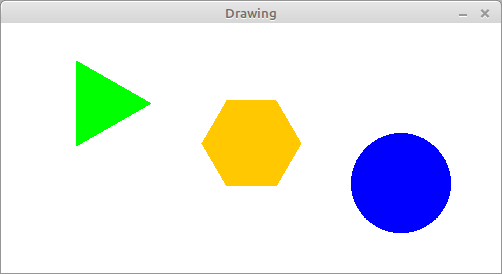
\includegraphics[width=4in]{figs/drawing.png}
\caption{Initial drawing of three \java{RegularPolygon} objects.}
\label{fig:drawing}
\end{center}
\end{figure}

%What's interesting about this example is that the polygon objects have methods from multiple classes.
%The constructor is defined in \java{RegularPolygon}.
%The \java{translate} method is defined in \java{Polygon}.
%The \java{draw} method (called by \java{paint}) is defined in \java{ColorPolygon}.
%And yet, everything works together seamlessly.


\section{Blinking Polygons}

At this point, we have a simple program that draws polygons.
We can make it a lot more fun by adding animation.
Chapter~\ref{conway} introduced the idea of simulating time steps.
We can write an animation loop at the end of \java{main}:

\begin{code}
while (true) {
    drawing.step();
    try {
        Thread.sleep(25);
    } catch (InterruptedException e) {
        // do nothing
    }
}
\end{code}

The \java{step} method of \java{Drawing} updates each polygon and repaints (clears and redraws) the canvas.

\begin{code}
public void step() {
    for (ColorPolygon cp : list) {
        cp.step();
    }
    repaint();
}
\end{code}

In order for this code to compile, ColorPolygon needs a \java{step} method too.
But it doesn't do anything yet; we'll override it in subclasses.

\begin{code}
public void step() {
    // do nothing
}
\end{code}

For example, we'll create a new type of polygon that blinks.
\java{BlinkingPolygon} add two more attributes to \java{RegularPolygon}: whether it is currently \java{visible}, and a time step \java{count}.

The constructor initializes these attributes after invoking \java{RegularPolygon}'s constructor (via \java{super}).
Initially, a \java{BlinkingPolygon} is visible, and its time step count is 0.

\begin{code}
public class BlinkingPolygon extends RegularPolygon {
    private boolean visible;
    private int count;

    public BlinkingPolygon(int nsides, int radius, Color c) {
        super(nsides, radius, c);
        visible = true;
        count = 0;
    }

    public void draw(Graphics g) {
        if (visible) {
            super.draw(g);
        }
    }

    public void step() {
        count++;
        if (count == 10) {
            count = 0;
            visible = !visible;
        }
    }
}
\end{code}

The \java{draw} method displays the polygon on the screen only if it is visible.
If not, then this polygon is not displayed.
The \java{step} method toggles the visibility flag every ten time steps.

You might notice something strange about this example.
\java{RegularPolygon}, the superclass, does not have a \java{draw} method.
So \java{super.draw} refers to the \java{draw} method in \java{ColorPolygon}.

%Replace \java{RegularPolygon} with \java{BlinkingPolygon} in the \java{main} method, and you will see Figure~\ref{fig:drawing} come to life.


\section{Java Interfaces}

You might be getting tired of polygons at this point.
Isn't it possible to draw anything else?
Of course the answer is ``yes'', but our \java{Drawing} is currently based on \java{ColorPolygon}.
In order to draw other types of objects, we'll need to generalize the code further.

The \java{Drawing} class does essentially three things: (1) it maintains a \java{list} of objects, (2) it invokes the \java{draw} method on each object, and (3) it invokes the \java{step} method on each object.
Here's one way to make it more general:

\begin{enumerate}

\item
Define a new parent class, named \java{Actor}, that provides the methods needed by \java{Drawing}:

\begin{code}
public class Actor {
    public void draw(Graphics g) {
        // do nothing
    }
    public void step() {
        // do nothing
    }
}
\end{code}

\item
In the \java{Drawing} class, find and replace ``\java{ColorPolygon}'' with ``\java{Actor}''.

\item
Any class that we want to draw will need to extend \java{Actor} (or one of its subclasses).

\end{enumerate}

There's just one problem: \java{ColorPolygon} already extends \java{Polygon}, and classes may extend only one superclass.
Not to mention that the \java{Actor} class seems pointless, given that it does nothing.

Java provides another mechanism for polymorphism that is more appropriate in this situation.
We can define \java{Actor} as an interface instead of a class:

\begin{code}
public interface Actor {
    void draw(Graphics g);
    void step();
}
\end{code}

An interface is a list of method declarations that define the capabilities of an object.
All methods are \java{public} by default, since they are intended to be invoked by other classes.

Interfaces require the keyword \java{implements} instead of \java{extends}.
We can change the definition of \java{ColorPolygon} as follows:

\begin{code}
public class ColorPolygon extends Polygon implements Actor
\end{code}

In terms of inheritance, \java{ColorPolygon} is both a \java{Polygon} and an \java{Actor}.
The same is true for subclasses of \java{ColorPolygon}.
As a result, the following statements are possible:

\begin{code}
Actor a1 = new ColorPolygon();
Actor a2 = new RegularPolygon(5, 50, Color.YELLOW);
Actor a3 = new BlinkingPolygon(8, 50, Color.RED);
\end{code}

Interfaces are another example of polymorphism.
The variables \java{a1}, \java{a2}, and \java{a3} are all different types of objects.
But each of them provides the \java{draw} and \java{step} methods as specified in the \java{Actor} interface.

Classes may extend only one superclass, but they may implement as many interfaces as they want.
We'll see an example with multiple interfaces in the next section.


\section{Event Listeners}

